\documentclass{article}
\usepackage[section]{placeins}
\usepackage{graphicx, wrapfig, amsmath, amssymb, physics, hyperref}
\hypersetup{
    colorlinks=true,
    linkcolor=blue,
    filecolor=magenta,      
    urlcolor=cyan,
    }

\author{Yaghoub Shahmari}
\title{Report - Problem Set No 5}
\date{\today}
\graphicspath{ {../Figs/} }

\begin{document}
    \maketitle
    \section*{Problem 1}
    \textbf{Basic description:}
    In this problem, we're going to discuss 2D Random Walkers. As the lecture notes described, we expect our results to show these relations:
    In my simulation value of the tau and l is equal to one. So we expect the simulation to show this:
    The simulation creates a list of random choices of walking and calculates the sum of total changes of location of the random walker. The number of chosen random steps is equal to t. We repeat the simulation for diffrent "t" many times and calculate gyration radius of total final position of each t.

    \textbf{Results:}

    % \begin{figure}[!htb]
    %     \centering
    %     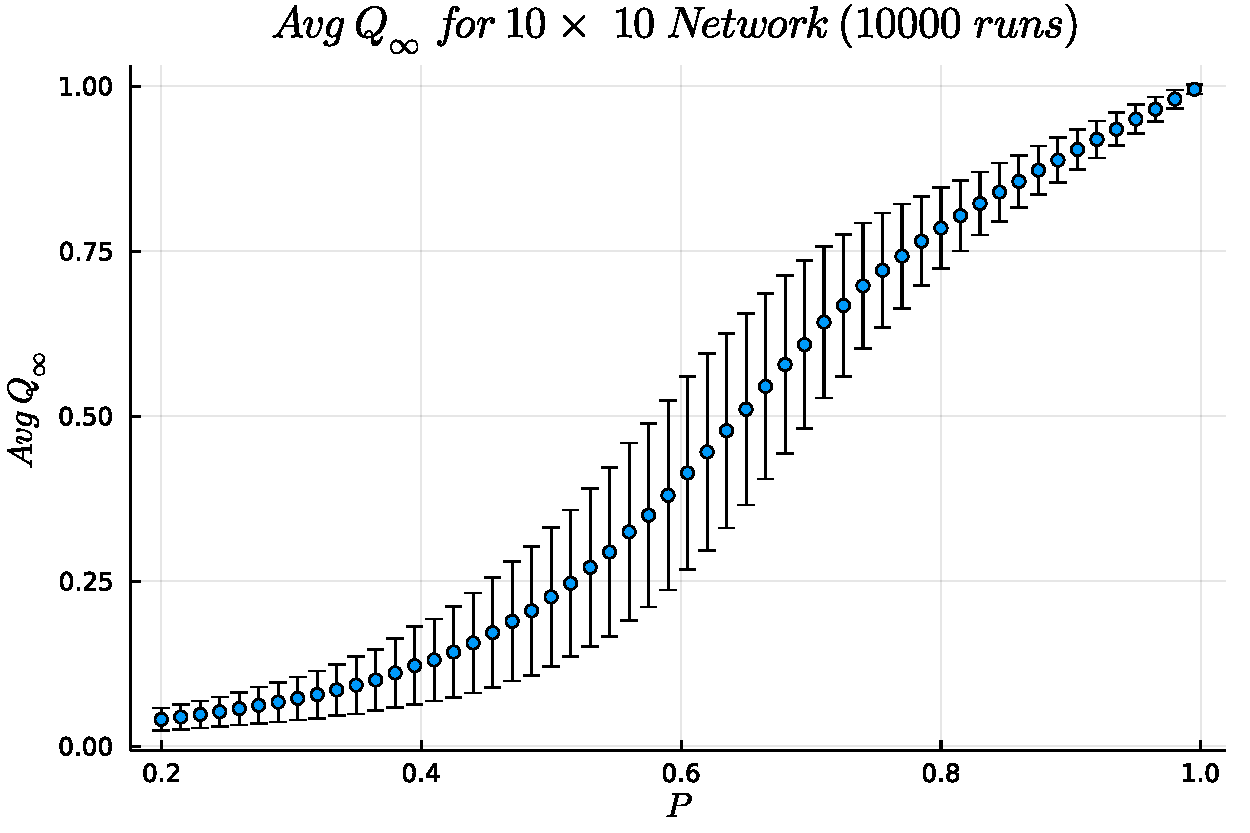
\includegraphics[scale = 0.275]{/Q1/dim10-10000}
    %     \label{fig:1.1}
    %     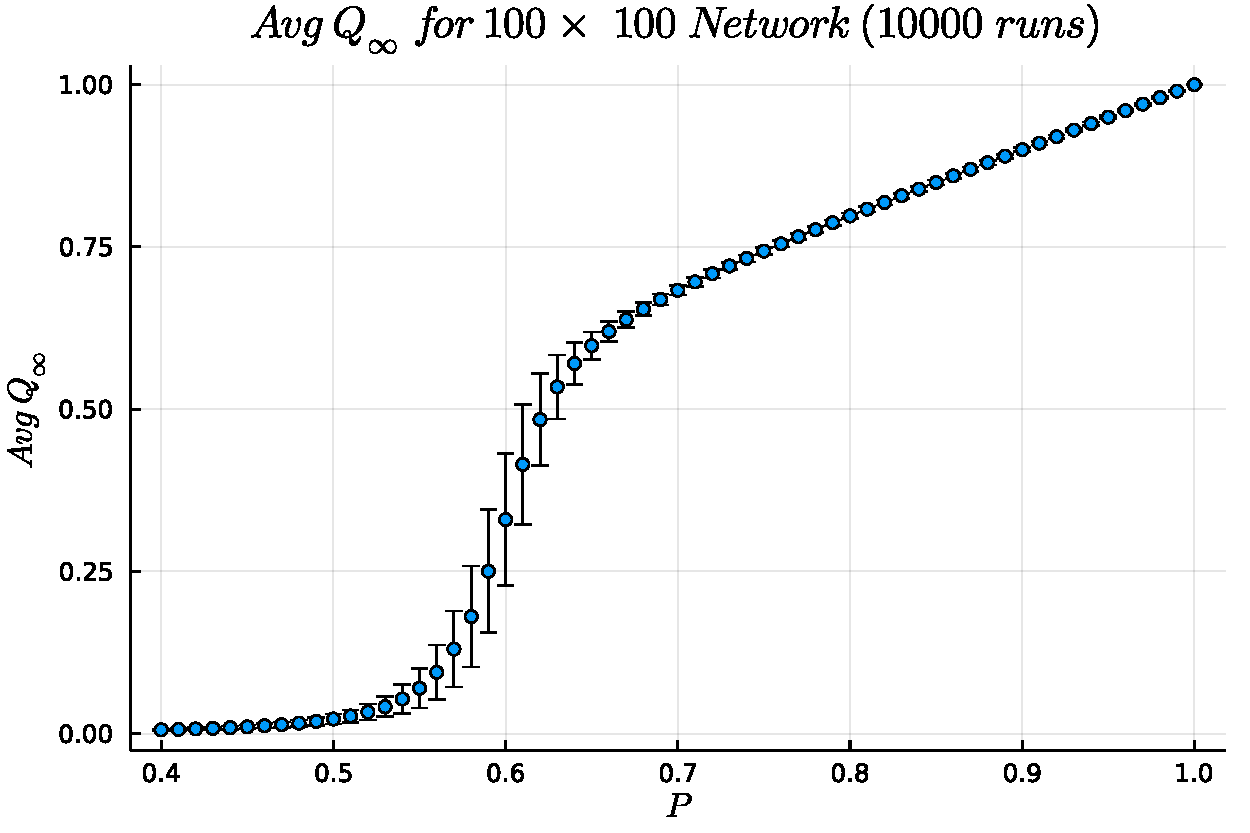
\includegraphics[scale = 0.275]{/Q1/dim100-10000}
    %     \label{fig:1.2}
    %     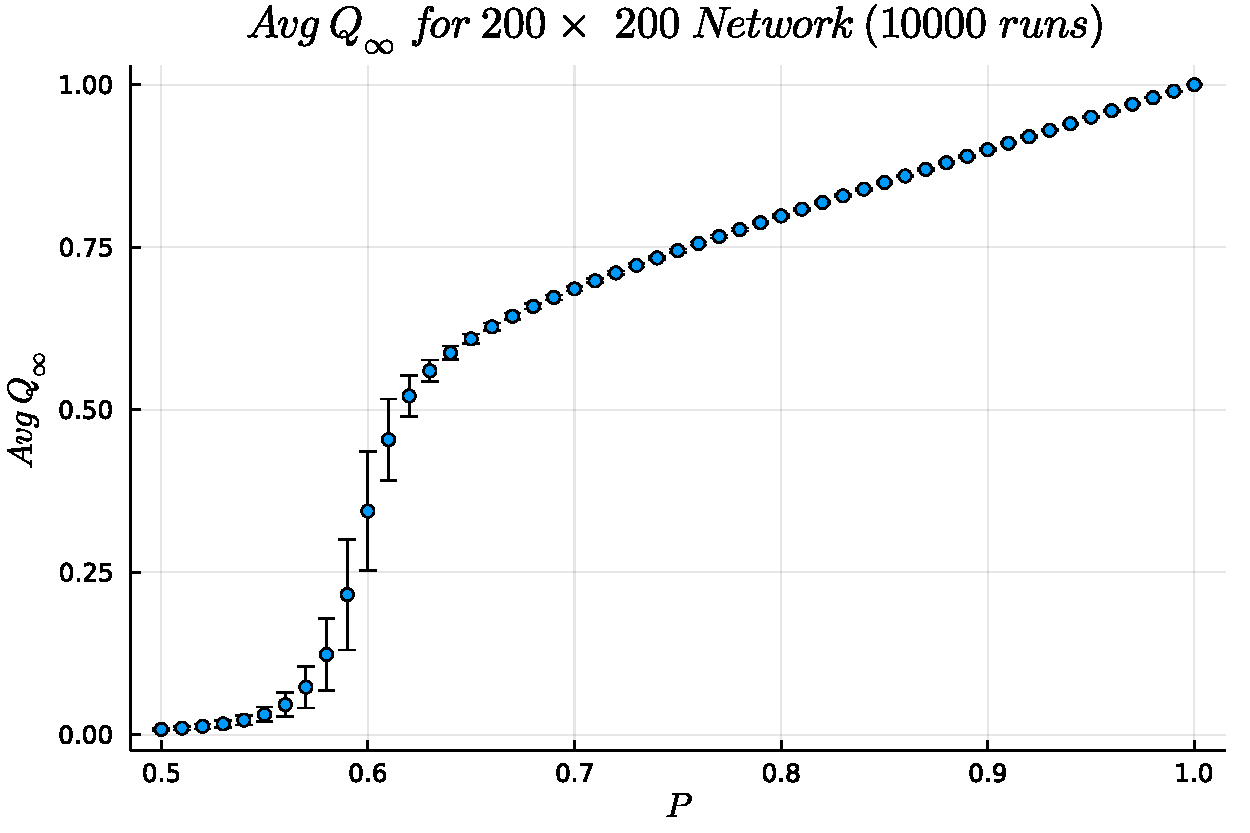
\includegraphics[scale = 0.4]{/Q1/dim200-10000}
    %     \label{fig:1.3}
    %     \caption{$Q_{\infty}$ for $L=10, 100, 200$}
    % \end{figure}

    \pagebreak

    \centering
    \textbf{The whole data I gathered is in \href{https://github.com/shahmari/ComputationalPhysics-Fall2021/tree/main/ProblemSet4/Data}{this link}}
    
    Thanks for watching :)
\end{document}